\documentclass[11pt,a4paper]{article}

% ============ PACKAGES ============
\usepackage[utf8]{inputenc}
\usepackage[T1]{fontenc}
\usepackage{lmodern}
\usepackage{geometry}
\usepackage{graphicx}
\usepackage{amsmath,amsfonts,amssymb}
\usepackage{booktabs}
\usepackage{float}
\usepackage{subcaption}
\usepackage{listings}
\usepackage{xcolor}
\usepackage{hyperref}
\usepackage{enumitem}
\usepackage{tikz}
\usepackage{array}
\usepackage{longtable}
\usepackage{multirow}
\usepackage{fancyhdr}
\usepackage{titlesec}
\usepackage{setspace}

% ============ PAGE SETUP ============
\geometry{left=2.5cm,right=2.5cm,top=2.5cm,bottom=2.5cm}
\onehalfspacing

% ============ CODE STYLE ============
\definecolor{codebg}{HTML}{f8f9fa}
\definecolor{codefg}{HTML}{212529}
\definecolor{keyword}{HTML}{0066cc}
\definecolor{string}{HTML}{228b22}
\definecolor{comment}{HTML}{6c757d}

\lstset{
    backgroundcolor=\color{codebg},
    basicstyle=\ttfamily\footnotesize\color{codefg},
    breaklines=true,
    captionpos=b,
    commentstyle=\color{comment}\itshape,
    frame=single,
    frameround=tttt,
    framexleftmargin=5mm,
    framexrightmargin=5mm,
    keywordstyle=\color{keyword}\bfseries,
    numbers=left,
    numbersep=10pt,
    numberstyle=\tiny\color{comment},
    stringstyle=\color{string},
    showstringspaces=false,
    tabsize=2,
    xleftmargin=2em,
    xrightmargin=2em
}

% ============ HYPERREF SETUP ============
\hypersetup{
    colorlinks=true,
    linkcolor=blue,
    filecolor=blue,
    urlcolor=blue,
    citecolor=blue,
    pdftitle={GRADEOPS Technical Report},
    pdfauthor={GRADEOPS Team},
    pdfsubject={AI-Powered Exam Grading System},
    pdfkeywords={AI, Grading, VLM, LLM, Education Technology}
}

% ============ HEADER/FOOTER ============
\pagestyle{fancy}
\fancyhf{}
\fancyhead[L]{\small\nouppercase{\leftmark}}
\fancyhead[R]{\small GRADEOPS Technical Report}
\fancyfoot[C]{\thepage}
\renewcommand{\headrulewidth}{0.4pt}
\renewcommand{\footrulewidth}{0.4pt}

% ============ TITLE ============
\title{
    \vspace{-1cm}
    {\Huge\textbf{GRADEOPS}}\\[0.5em]
    {\Large\color{gray}AI-Powered Exam Grading System}\\[2em]
    {\large Technical Report}\\[0.5em]
    {\normalsize\today}
}
\author{System Architecture \& Implementation}
\date{}

% ===================================================================
\begin{document}
\maketitle
\thispagestyle{empty}
\newpage

% ============ ABSTRACT ============
\begin{abstract}
\noindent
GRADEOPS is a production-ready, Human-in-the-Loop (HITL) grading pipeline that leverages Vision-Language Models (VLMs) for optical character recognition on handwritten exam scans and Large Language Model (LLM) agents for automated evaluation against instructor-defined rubrics. The system enables Teaching Assistants (TAs) to rapidly review and validate AI-generated grades through an intuitive web dashboard, ensuring accuracy and fairness. This report details the system architecture, database schema, API design, AI engine, frontend implementation, and deployment strategy.
\end{abstract}

\tableofcontents
\newpage

% ===================================================================
\section{Introduction}
\label{sec:introduction}

% ----------
\subsection{Background and Motivation}
Manual grading of exams is a labor-intensive process that involves hours of repetitive work for instructors and teaching assistants. For large classes with hundreds of students, the grading workload becomes a significant bottleneck, detracting from time available for student engagement and curriculum development. Furthermore, maintaining consistency across graders is challenging, potentially leading to unfair grade disparities.

The integration of artificial intelligence into educational workflows has opened new possibilities for automating and augmenting the grading process. However, fully automated systems lack the human judgment necessary to handle edge cases, partial credit, and nuanced responses. A Human-in-the-Loop (HITL) approach, where AI handles the initial grading and human reviewers validate the results, offers a balanced solution that combines the efficiency of automation with the reliability of human oversight.

% ----------
\subsection{Project Objectives}
The primary objectives of GRADEOPS are:

\begin{enumerate}[leftmargin=2em]
    \item \textbf{Automate Initial Grading}: Use VLMs to extract text from handwritten exam scans and LLM agents to grade responses against configurable rubrics.
    \item \textbf{Enable Human Review}: Provide TAs with a streamlined dashboard for reviewing AI grades, with one-click approval or override capabilities.
    \item \textbf{Ensure Consistency}: Define strict rubric criteria with partial credit support to minimize inter-grader variability.
    \item \textbf{Support Scalability}: Handle large exam volumes with batch processing and asynchronous job execution.
    \item \textbf{Monitor System Health}: Offer real-time analytics and health monitoring for administrators.
\end{enumerate}

% ----------
\subsection{Report Structure}
This technical report is organized as follows: Section \ref{sec:architecture} describes the overall system architecture and technology stack; Section \ref{sec:backend} details the backend implementation, including the database schema and AI engine; Section \ref{sec:frontend} covers the frontend design and user experience; Section \ref{sec:api} documents the REST API endpoints; Section \ref{sec:deployment} outlines the deployment strategy; and Section \ref{sec:conclusion} provides concluding remarks and future work.

% ===================================================================
\newpage
\section{System Architecture}
\label{sec:architecture}

% ----------
\subsection{High-Level Design}
GRADEOPS follows a three-tier architecture pattern consisting of a presentation layer (frontend), application layer (backend API), and data layer (database and file storage). Figure \ref{fig:architecture} illustrates the high-level component diagram.

\begin{figure}[H]
    \centering
    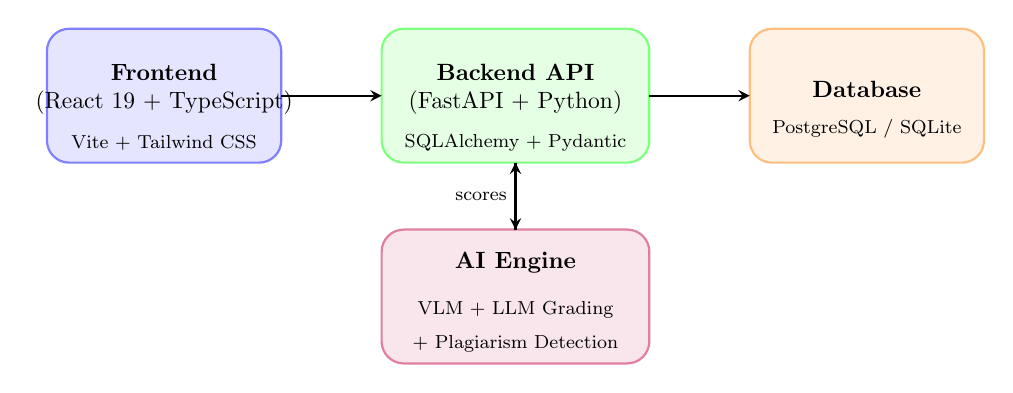
\begin{tikzpicture}[scale=0.85, transform shape]
        % Frontend Box
        \draw[rounded corners=8pt, fill=blue!10, draw=blue!50, thick] (0,0) rectangle (3.5,2);
        \node[align=center] at (1.75,1.1) {\textbf{Frontend}\\(React 19 + TypeScript)};
        \node[align=center] at (1.75,0.3) {\footnotesize Vite + Tailwind CSS};

        % Backend Box
        \draw[rounded corners=8pt, fill=green!10, draw=green!50, thick] (5,0) rectangle (9,2);
        \node[align=center] at (7,1.1) {\textbf{Backend API}\\(FastAPI + Python)};
        \node[align=center] at (7,0.3) {\footnotesize SQLAlchemy + Pydantic};

        % Database Box
        \draw[rounded corners=8pt, fill=orange!10, draw=orange!50, thick] (10.5,0) rectangle (14,2);
        \node[align=center] at (12.25,1.1) {\textbf{Database}};
        \node[align=center] at (12.25,0.5) {\footnotesize PostgreSQL / SQLite};

        % AI Engine Box
        \draw[rounded corners=8pt, fill=purple!10, draw=purple!50, thick] (5,-3) rectangle (9,-1);
        \node[align=center] at (7,-1.5) {\textbf{AI Engine}};
        \node[align=center] at (7,-2.2) {\footnotesize VLM + LLM Grading};
        \node[align=center] at (7,-2.7) {\footnotesize + Plagiarism Detection};

        % Arrows
        \draw[->, thick, >=stealth] (3.5,1) -- (5,1);
        \draw[->, thick, >=stealth] (9,1) -- (10.5,1);
        \draw[->, thick, >=stealth] (7,0) -- (7,-1);
        \draw[->, thick, >=stealth, dashed] (7,-1) -- (7,0) node[midway, left] {\footnotesize scores};
    \end{tikzpicture}
    \caption{High-level system architecture diagram showing the three-tier design and AI engine integration.}
    \label{fig:architecture}
\end{figure}

% ----------
\subsection{Technology Stack}
\label{subsec:tech-stack}

Table \ref{tab:tech-stack} summarizes the technology stack used across the project.

\begin{table}[H]
    \centering
    \caption{Technology stack summary}
    \label{tab:tech-stack}
    \begin{tabular}{@{}lll@{}}
        \toprule
        \textbf{Layer} & \textbf{Technology} & \textbf{Purpose} \\
        \midrule
        Frontend & React 19 + TypeScript & UI framework and type safety \\
        Frontend & Tailwind CSS & Utility-first styling \\
        Frontend & Vite & Build tool and dev server \\
        Backend & FastAPI & Async web framework \\
        Backend & SQLAlchemy & ORM and database abstraction \\
        Backend & Pydantic & Data validation and settings \\
        Backend & PyMuPDF & PDF processing \\
        AI & OpenCV & Image preprocessing \\
        AI & Sentence-Transformers & Semantic similarity \\
        Database & SQLite / PostgreSQL & Data persistence \\
        DevOps & Docker + Compose & Container orchestration \\
        \bottomrule
    \end{tabular}
\end{table}

% ----------
\subsection{System Components}

% --- Frontend ---
\subsubsection{Frontend Application}
The frontend is a single-page application (SPA) built with React 19 and TypeScript, compiled by Vite. It provides three role-based views:

\begin{itemize}[leftmargin=2em]
    \item \textbf{Instructor Portal}: Upload exam PDFs, configure rubric criteria, and initiate grading.
    \item \textbf{TA Review Dashboard}: Review AI-generated grades with extracted text, justification, and image previews; approve or override scores.
    \item \textbf{Admin Dashboard}: Monitor system statistics, storage usage, and health metrics.
\end{itemize}

All components are styled with Tailwind CSS, ensuring a consistent, responsive, and modern user interface.

% --- Backend ---
\subsubsection{Backend API Service}
The backend is built with FastAPI, a high-performance async Python web framework. It exposes RESTful endpoints for all system operations, structured into modular routers:

\begin{itemize}[leftmargin=2em]
    \item \texttt{upload}: File upload and management
    \item \texttt{config}: Course, exam, and rubric configuration
    \item \texttt{grade}: Grading pipeline execution
    \item \texttt{review}: TA review and approval workflows
    \item \texttt{monitor}: System statistics and health monitoring
\end{itemize}

% --- AI Engine ---
\subsubsection{AI Grading Engine}
The AI engine comprises three core components:

\begin{enumerate}[leftmargin=2em]
    \item \textbf{VLMExtractor}: Extracts handwritten text from answer images using Vision-Language Models (mock implementation for development with real VLM integration planned).
    \item \textbf{GradingAgent}: Evaluates extracted text against rubric criteria using keyword matching and heuristic scoring, with LLM integration planned for production.
    \item \textbf{PlagiarismDetector}: Computes semantic similarity between student responses using sentence embeddings to identify potential plagiarism.
\end{enumerate}

% --- Database ---
\subsubsection{Database Layer}
The database layer uses SQLAlchemy as the ORM, supporting both SQLite (development) and PostgreSQL (production). The schema defines entities for users, courses, exams, rubrics, submissions, answers, and reviews, as detailed in Section \ref{subsec:database-schema}.

% ===================================================================
\newpage
\section{Backend Implementation}
\label{sec:backend}

% ----------
\subsection{Database Schema}
\label{subsec:database-schema}

The database schema is designed to support the complete exam grading workflow, from course creation through final review. Figure \ref{tab:schema} presents the entity-relationship mapping.

\begin{table}[H]
    \centering
    \caption{Database schema entities}
    \label{tab:schema}
    \begin{tabular}{@{}lp{9cm}@{}}
        \toprule
        \textbf{Entity} & \textbf{Description} \\
        \midrule
        \textbf{User} & System users with roles (instructor, ta, admin). Username is unique. \\
        \textbf{Course} & A course entity, linked to an instructor via foreign key. \\
        \textbf{Exam} & An exam within a course. Contains rubrics and submissions. \\
        \textbf{Rubric} & Grading criteria for a specific question, stored as JSON with max score. \\
        \textbf{Submission} & A student's exam submission (PDF file). Linked to an exam. \\
        \textbf{Answer} & An individual question response, linked to a submission and rubric. Stores extracted text, AI score, and final score. \\
        \textbf{Review} & TA review record for an answer, with optional override and comments. \\
        \bottomrule
    \end{tabular}
\end{table}

% ----------
\subsection{SQLAlchemy Models}

The SQLAlchemy ORM models define the Python representation of the database schema. Key relationships include:

\begin{lstlisting}[language=Python, caption={SQLAlchemy ORM model definitions}]
class User(Base):
    __tablename__ = "users"
    id = Column(Integer, primary_key=True)
    username = Column(String, unique=True)
    role = Column(String)  # 'instructor' or 'ta'

class Course(Base):
    __tablename__ = "courses"
    id = Column(Integer, primary_key=True)
    title = Column(String)
    instructor_id = Column(Integer, ForeignKey("users.id"))

class Exam(Base):
    __tablename__ = "exams"
    id = Column(Integer, primary_key=True)
    title = Column(String)
    course_id = Column(Integer, ForeignKey("courses.id"))

class Rubric(Base):
    __tablename__ = "rubrics"
    id = Column(Integer, primary_key=True)
    exam_id = Column(Integer, ForeignKey("exams.id"))
    question_number = Column(String)
    max_score = Column(Float)
    criteria = Column(JSON)  # Structured grading rules

class Submission(Base):
    __tablename__ = "submissions"
    id = Column(Integer, primary_key=True)
    exam_id = Column(Integer, ForeignKey("exams.id"))
    student_id = Column(String)
    pdf_path = Column(String)
    uploaded_at = Column(DateTime, default=datetime.utcnow)

class Answer(Base):
    __tablename__ = "answers"
    id = Column(Integer, primary_key=True)
    submission_id = Column(Integer, ForeignKey("submissions.id"))
    rubric_id = Column(Integer, ForeignKey("rubrics.id"))
    image_path = Column(String)
    extracted_text = Column(Text, nullable=True)
    ai_score = Column(Float, nullable=True)
    ai_justification = Column(JSON, nullable=True)
    final_score = Column(Float, nullable=True)
    status = Column(String, default="pending")

class Review(Base):
    __tablename__ = "reviews"
    id = Column(Integer, primary_key=True)
    answer_id = Column(Integer, ForeignKey("answers.id"))
    is_overridden = Column(Boolean, default=False)
    comments = Column(Text, nullable=True)
    reviewed_at = Column(DateTime, default=datetime.utcnow)
\end{lstlisting}

% ----------
\subsection{AI Engine}
\label{subsec:ai-engine}

% --- VLM ---
\subsubsection{Vision-Language Model Text Extraction}
The \texttt{VLMExtractor} class handles text extraction from answer images. For development, it uses a mock implementation that returns placeholder text. In production, this will be replaced with a real VLM (e.g., Qwen-VL 7B or Claude Vision).

\begin{lstlisting}[language=Python, caption={VLM text extraction interface}]
class VLMExtractor:
    def __init__(self, model_name: str = "qwen-vl"):
        self.model_name = model_name
        self.is_mock = True

    def extract_text(self, image_path: str) -> str:
        if self.is_mock:
            return self._extract_text_mock(image_path)
\end{lstlisting}

% --- Grading ---
\subsubsection{Agentic Grading}
The \texttt{GradingAgent} evaluates extracted text against rubric criteria. Each criterion is checked against the student's response using a keyword matching heuristic, awarding points if the response contains a sufficient number of matching keywords (60\% threshold).

\begin{lstlisting}[language=Python, caption={Grading logic}]
def grade_answer(self, extracted_text: str, rubric: Dict):
    justification = {}
    total_score = 0.0

    for i, (criterion_key, criterion) in enumerate(
            criteria.items(), 1):
        condition = criterion.get("condition", "")
        points = criterion.get("points", 0)

        met = self._evaluate_condition(condition, extracted_text)
        justification[f"criterion_{i}"] = {
            "condition": condition,
            "met": met,
            "score_awarded": points if met else 0,
        }
        if met:
            total_score += points

    return {
        "score": total_score,
        "justification": justification,
        "success": True
    }
\end{lstlisting}

The grading also generates performance-based feedback categories: ``Excellent'' ($\geq$90\%), ``Good'' (80--89\%), ``Satisfactory'' (70--79\%), ``Passing'' (60--69\%), and ``Needs Improvement'' ($<$60\%).

% --- Plagiarism ---
\subsubsection{Plagiarism Detection}
The \texttt{PlagiarismDetector} computes semantic similarity between pairs of student answers using sentence embeddings. A pair is flagged as suspicious if the similarity exceeds a configurable threshold (default 0.85).

% ----------
\subsection{Router Implementations}

% --- Upload ---
\subsubsection{Upload Router}
Handles exam PDF uploads and auto-triggers the grading pipeline. Files are stored in a designated uploads directory, and answers are extracted and stored with the ``pending'' status.

% --- Grade ---
\subsubsection{Grade Router}
Manages the grading workflow:

\begin{itemize}[leftmargin=2em]
    \item \texttt{POST /grade/{answer\_id}/trigger}: Manually triggers grading for a single answer.
    \item \texttt{GET /grade/status/{answer\_id}}: Checks the grading status of an answer.
    \item \texttt{POST /grade/batch/trigger}: Triggers batch grading across multiple submissions.
\end{itemize}

Grading is performed in a background task to prevent blocking the API response.

% --- Review ---
\subsubsection{Review Router}
Provides TA-facing endpoints:

\begin{itemize}[leftmargin=2em]
    \item \texttt{GET /review/pending}: Returns all answers with ``graded'' status for review.
    \item \texttt{POST /review/{answer\_id}/approve}: Approves the AI grade.
    \item \texttt{POST /review/{answer\_id}/override}: Overrides with a new score and optional comments.
    \item \texttt{GET /review/plagiarism-check/{exam\_id}}: Runs plagiarism detection across an exam.
\end{itemize}

% --- Monitor ---
\subsection{Monitoring and Health}
The \texttt{monitor} router provides system statistics including storage usage, submission counts by status, and per-exam analytics. The health check endpoint (\texttt{GET /health}) verifies database connectivity and storage health.

% ----------
\subsection{Configuration Management}

Pydantic-based configuration manages environment-specific settings:

\begin{lstlisting}[language=Python, caption={Pydantic settings configuration}]
class Settings(BaseSettings):
    database_url: str = "sqlite:///./gradeops.db"
    api_title: str = "GRADEOPS API"
    api_version: str = "1.0.0"
    upload_dir: str = "uploads"
    artifacts_dir: str = "artifacts"
    vlm_model: Literal["qwen-vl", "gpt-4-vision", "claude-3"] = "qwen-vl"
    similarity_threshold: float = 0.85
    log_level: str = "INFO"
\end{lstlisting}

% ===================================================================
\newpage
\section{Frontend Implementation}
\label{sec:frontend}

% ----------
\subsection{Technology Choices}
The frontend is built with modern web technologies chosen for their performance, developer experience, and ecosystem maturity:

\begin{itemize}[leftmargin=2em]
    \item \textbf{React 19}: Latest React with automatic batching and improved Concurrent Features.
    \item \textbf{TypeScript}: Type-safe development with autocomplete and compile-time error checking.
    \item \textbf{Tailwind CSS}: Utility-first styling for rapid, consistent UI development.
    \item \textbf{Vite}: Hot Module Replacement (HMR) and fast production builds.
\end{itemize}

% ----------
\subsection{Application Structure}

The frontend consists of a single \texttt{App.tsx} entry point that manages role-based routing and three main components:

% ----------
\subsection{Component Design}

% --- App ---
\subsubsection{App.tsx (Role Selection)}
The entry point provides a dark-themed, modern role selection screen. Key features include:

\begin{itemize}[leftmargin=2em]
    \item Gradient background with radial glow effects for visual depth.
    \item Animated cards with hover lift, glow rings, and directional chevrons.
    \item Backend health checking with soft amber warning indicators.
    \item Glassmorphism header with backdrop blur and role badge indicators.
\end{itemize}

% --- UploadPortal ---
\subsubsection{UploadPortal Component}
The instructor interface supports:

\begin{itemize}[leftmargin=2em]
    \item Multi-section form with numbered steps (Exam Details, Rubric Criteria, File Upload).
    \item Dynamic rubric management: add, edit, and remove criteria with condition and point values.
    \item Drag-and-drop file upload with visual state feedback.
    \item File list with status icons (pending, uploading, done, error) and per-file removal.
    \item Overall upload progress bar and per-file status tracking.
\end{itemize}

Rubric criteria are state-managed with unique IDs generated via \texttt{crypto.randomUUID}.

% --- ReviewDashboard ---
\subsubsection{ReviewDashboard Component}
The TA review interface is optimized for speed with:

\begin{itemize}[leftmargin=2em]
    \item Two-pane layout: Student answer (left), AI grading panel (right).
    \item Submission navigation with progress bar and prev/next buttons.
    \item Score visualization with color-coded progress bars (red/amber/emerald).
    \item Keyboard shortcuts: Enter to approve, arrow keys to navigate.
    \item Approval feedback toasts for success/error states.
    \item Auto-refresh toggle with configurable polling interval.
\end{itemize}

% --- AdminDashboard ---
\subsubsection{AdminDashboard Component}
The administrator view includes:

\begin{itemize}[leftmargin=2em]
    \item Overview stat cards with colorful icons, values, and percentage badges.
    \item Overall progress bar showing graded proportion across all answers.
    \item Storage usage panel with animated progress bars.
    \item System health indicators with animated status pulses.
\end{itemize}

% ----------
\subsection{Styling and Animation}
Custom CSS animations are defined in \texttt{index.css} for consistent transitions across the application:

\begin{itemize}[leftmargin=2em]
    \item \texttt{fadeInUp}: Smooth upward entry animation.
    \item \texttt{fadeIn}: General opacity transition.
    \item \texttt{slideInRight}: Right-to-left panel transition.
    \item \texttt{pulse-ring}: Attention-gathering pulsating ring.
    \item \texttt{scrollbar-thin}: Custom thin scrollbar styling.
\end{itemize}

% ===================================================================
\newpage
\section{API Documentation}
\label{sec:api}

% ----------
\subsection{Endpoint Overview}

Table \ref{tab:api-endpoints} summarizes the available API endpoints organized by router.

\begin{longtable}{@{}llp{6cm}@{}}
    \caption{API endpoint summary} \label{tab:api-endpoints} \\
    \toprule
    \textbf{Method} & \textbf{Endpoint} & \textbf{Description} \\
    \midrule
    \endfirsthead
    \multicolumn{3}{c}{\tablename\ \thetable{} -- continued from previous page} \\
    \toprule
    \textbf{Method} & \textbf{Endpoint} & \textbf{Description} \\
    \midrule
    \endhead
    \bottomrule
    \endfoot
    % Auth
    POST & /auth/login & Authenticate user (mock) \\
    % Config
    POST & /config/course/ & Create new course \\
    GET & /config/course/ & List all courses \\
    POST & /config/exam/ & Create new exam \\
    GET & /config/exam/ & List exams by course \\
    POST & /config/rubric/ & Create grading rubric \\
    GET & /config/rubric/exam/{exam\_id} & Get rubrics for an exam \\
    PUT & /config/rubric/{rubric\_id} & Update rubric \\
    DELETE & /config/rubric/{rubric\_id} & Delete rubric \\
    % Upload
    POST & /upload/submission/ & Upload student exam PDF \\
    GET & /upload/submission/{submission\_id} & Get submission details \\
    GET & /upload/exam/{exam\_id}/submissions & List submissions \\
    % Grade
    POST & /grade/{answer\_id}/trigger & Trigger grading for answer \\
    GET & /grade/status/{answer\_id} & Get grading status \\
    POST & /grade/batch/trigger & Batch grading \\
    % Review
    GET & /review/pending & Get pending answers \\
    GET & /review/pending-count & Count pending \\
    POST & /review/{answer\_id}/approve & Approve AI grade \\
    POST & /review/{answer\_id}/override & Override with comments \\
    GET & /review/plagiarism-check/{exam\_id} & Check plagiarism \\
    GET & /review/{answer\_id}/details & Full answer details \\
    % Monitor
    GET & /health & Health check \\
    GET & /monitor/stats & System statistics \\
    GET & /monitor/submissions-by-status & Status breakdown \\
    GET & /monitor/exam-summary/{exam\_id} & Exam analytics \\
\end{longtable}

% ----------
\subsection{Request and Response Formats}
All API responses follow a consistent JSON structure:

\begin{lstlisting}[language=JSON, caption={Standard response format}]
{
  "data": {},
  "error": null,
  "status_code": 200
}
\end{lstlisting}

Error responses include descriptive detail and, in debug mode, the underlying error trace.

% ----------
\subsection{Health Check Endpoint}
The health endpoint provides real-time system status:

\begin{lstlisting}[language=JSON, caption={Health check response}]
{
  "status": "healthy",
  "database": "connected",
  "storage": {
    "upload_dir_size": 1024000,
    "artifacts_dir_size": 2048000,
    "disk_percent": 50.0
  }
}
\end{lstlisting}

% ===================================================================
\newpage
\section{Deployment and Operations}
\label{sec:deployment}

% ----------
\subsection{Docker Configuration}
The project includes a \texttt{docker-compose.yml} file orchestrating three services:

\begin{itemize}[leftmargin=2em]
    \item \textbf{Backend}: Python FastAPI application with hot-reload for development.
    \item \textbf{Frontend}: React SPA served on port 3000.
    \item \textbf{Database}: PostgreSQL 15 Alpine with persistent volume.
\end{itemize}

% ----------
\subsection{Environment Configuration}
Production deployment requires the following environment variables:

\begin{lstlisting}[caption={Environment variables}]
DATABASE_URL=postgresql://gradeops:gradeops@db:5432/gradeops
DEBUG=false
LOG_LEVEL=INFO
VLM_MODEL=qwen-vl
OPENAI_API_KEY=sk-...
\end{lstlisting}

% ----------
\subsection{Production Considerations}

Key production recommendations include:

\begin{enumerate}[leftmargin=2em]
    \item Use PostgreSQL instead of SQLite for concurrent access.
    \item Disable debug mode and set logging to WARN.
    \item Configure a reverse proxy (nginx) for SSL termination and CORS.
    \item Implement real JWT authentication instead of mock tokens.
    \item Enable HTTPS with proper certificate management.
    \item Configure GPU resources for VLM inference.
    \item Set up log aggregation and monitoring (e.g., ELK stack, Prometheus).
\end{enumerate}

% ===================================================================
\newpage
\section{Conclusion and Future Work}
\label{sec:conclusion}

% ----------
\subsection{Summary}
GRADEOPS presents a comprehensive solution to the challenge of scaling exam grading. By combining Vision-Language Models for text extraction, LLM agents for automated evaluation, and a streamlined Human-in-the-Loop review process, the system achieves a balance between automation efficiency and grading accuracy. The modular architecture allows for easy integration of production-grade AI models, while the web-based dashboards ensure accessibility for all user roles.

% ----------
\subsection{Future Enhancements}
Planned improvements include:

\begin{enumerate}[leftmargin=2em]
    \item \textbf{Real VLM Integration}: Replace mock extractor with Qwen-VL 7B or Claude Vision for production-grade OCR.
    \item \textbf{LLM Function Calling}: Implement real LLM grading with structured function calling for precise rubric evaluation.
    \item \textbf{Batch Processing}: Add Celery + Redis for asynchronous background job processing at scale.
    \item \textbf{Email Notifications}: Automated notifications for instructors when grading is complete.
    \item \textbf{LMS Integration}: Export grades to CSV and integrate with learning management systems.
    \item \textbf{Student Appeals}: Workflow for students to challenge grades with human review.
    \item \textbf{Mobile Application}: Native mobile app for TAs to review on the go.
    \item \textbf{Advanced Analytics}: Fairness metrics and bias detection in AI grading.
    \item \textbf{Multi-language Support}: Process exams in multiple languages.
\end{enumerate}

% ===================================================================
\newpage
\appendix
\section{File Structure}

\begin{lstlisting}[caption={Project directory structure}]
gradeops/
├── backend/
│   ├── main.py              # FastAPI application entry
│   ├── models.py            # SQLAlchemy ORM models
│   ├── schemas.py           # Pydantic request/response schemas
│   ├── database.py          # Database engine and session
│   ├── config.py            # Application settings
│   ├── logger.py            # Logging configuration
│   ├── ai_engine.py         # VLM + LLM + Plagiarism
│   ├── utils.py             # PDF and file utilities
│   └── routers/
│       ├── upload.py        # File upload endpoints
│       ├── config.py        # Course/exam/rubric endpoints
│       ├── grade.py         # Grading pipeline endpoints
│       ├── review.py        # TA review endpoints
│       └── monitor.py       # Admin monitoring endpoints
├── frontend/
│   ├── src/
│   │   ├── index.css        # Global styles and animations
│   │   ├── App.tsx          # Main app and role routing
│   │   └── components/
│   │       ├── UploadPortal.tsx      # Instructor interface
│   │       ├── ReviewDashboard.tsx     # TA review dashboard
│   │       └── AdminDashboard.tsx      # Admin monitoring
├── docker-compose.yml
├── API.md
├── IMPROVEMENTS.md
└── README.md
\end{lstlisting}

% ===================================================================
\end{document}
